%file included in thesis.tex

\chapter{Implementation}
In this chapter implementation specific issues are treated. Figure
\ref{chap6:fig-implementation} shows the three-layer implementation of the project.
\begin{figure}[htbp]
    \centering
    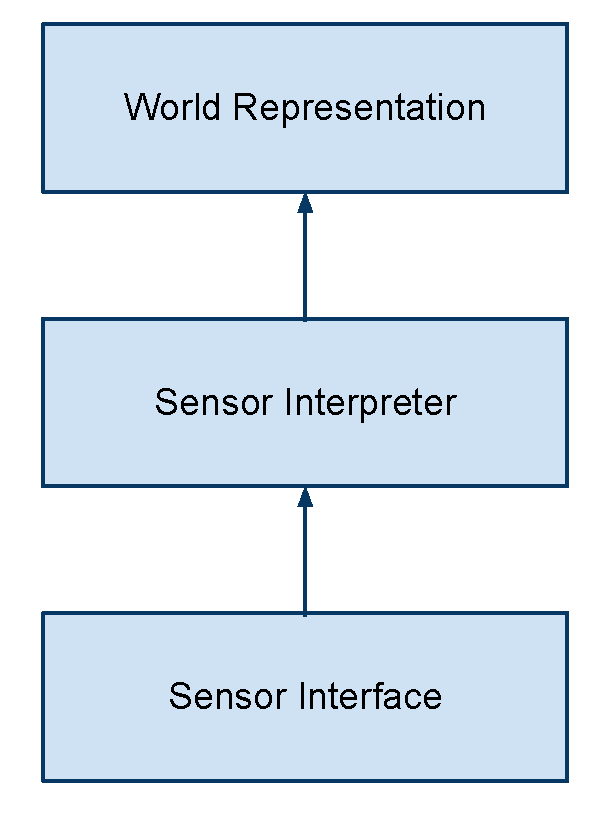
\includegraphics[width=0.4\textwidth]{pics/implementation}
    \caption{Three-layer implementation}
    \label{chap6:fig-implementation}
\end{figure}
The \emph{low-level} layer reads and converts the raw sensor data into common data which can be
interpreted by the \emph{middle} layer. This layer handles all the ''washing`` of the
sensor data, and applies the reasoning and tries to recognize the environment. The third
and last layer is the \emph{world} layer which handles the global data, where the robot is
and where it should move next. 

The project is implemented in both \emph{C/C++} and Matlab. The sensor layer are
implemented in \emph{C/C++} while the other layers are implemented in Object-Oriented
Matlab. 

\section{Low-level Interfaces}
The low-level interfaces from the sensors are implemented in \emph{C/C++} and uses the
supplied sensor APIs. The SwissRanger 3000 API were used directly in Matlab. The Hokuyo
API was a little more tricky to use. A Matlab interface function were implemented to get
the sensor data directly into Matlab.

\subsection{Stereo Camera Implementation}
For the stereo camera, a program was written using the \emph{OpenCV} library. A open
source computer vision library, initially developed by Intel. This library have many
excellent and optimized functions for grabbing images, camera calibration, image rectification
and stereo matching. This produced a disparity map, which again where reprojected into 3D
by the \emph{cvReprojectTo3D()}-function. This coordinate images where saved to disk and
read into Matlab for further processing. 

\begin{algorithm}
\caption{The Stereo Capture Procedure}
\label{chap6:alg-stereomatch}
    \begin{algorithmic}
    \STATE \textbf{begin}
    \STATE Connect to Cameras
    \FOR{no of images $<$ 20}
        \STATE Capture images of Checkerboard and find corners
    \ENDFOR
    \STATE Calculate the distortion parameters using Healy's Method.
    \WHILE{Not Quitting}
        \STATE Capture images
        \STATE Rectify Images
        \STATE Stereo matching using Block Matching 
        \STATE Reproject disparity map to 3DImage
        \STATE Dump 3D Coordinates to Disk
    \ENDWHILE
    \STATE \textbf{end}
    \end{algorithmic}
\end{algorithm}
This program calibrates the cameras, rectifies the images, finds stereo correspondences
and reprojects them to 3D coordinates.


\section{Mid-level Implantations}
The middle layers goal is to process and interpret the sensor data to best ability. This
layer is in charge of doing the reasoning, and draw out important information form the
sensor data. The main task is to find lines in the 2D sensor data, and cylinder shapes in
the 3D data. 

\subsection{Analysis of 3D Sensor Data}



\subsubsection{Filtering of ToF Data}


\subsubsection{Surface Fit Algorithm}


\paragraph{Guass-Newton Least Squares}


\paragraph{Issues}
The algorithm is sensitive to edge data. This can be controlled with limiting the interval
in the z-direction of which the cylinder is fitted to the data.*************FIX*******


\section{High-level Implementations}

\subsection{World Representation}
The world representation are implemented as objects in Matlab.




